
\section{Evaluation}
\label{sect:exper}

We have implemented and evaluated a prototype of our VO scheme on a Linux cluster
of 8-core AMD FX-8120 at 3.1 GHz with 16 GB RAM. 
Our implementation is based on Alibaba's Xen cloud platform~\cite{Aliyun,WeiZhangIEEE}.
Each machine  is equiped with a 
a distributed file system (QFS) running in the cluster manages six 3TB disks
with default replication degree set to 3. The CDS replication is set to 5.
Objectives of our evaluation are:
1) Study the deduplication efficiency of the VC approach and compare with an alternative
design.
2) Evaluate the backup throughput performance VC  for a large number of VMs.
%Compare with the data domain approach~\cite{bottleneck08}.
3) Examine the impacts of VC for fault isolation. 

%\section{Experiments}
%Our main test-bed is an cluster of 6 machines,
%Our data set consists of 350 virtual machine image snapshots taken from Alibaba.com's
%public VM cloud in China. 
%We select 35 VMs from the most popular 7 OSes: 
%Debian, Ubuntu, Redhat, CentOS, Win2003 32bit, win2003 64 bit and win2008 64 bit. 
%For each OS, 5 VMs are chosen, and every VM come with 10 full snapshots.
%\subsection{Experimental setup}

\comments{
%We are running our deduplication/backup  service on 100 nodes.
%Memory usage is about 150MB space per node during backup and
%the CPU usage is very small during the experiments. 
We have performed a trace-driven study using  a 1323 VM dataset  collected from 
%100 Alibaba Aliyun's cloud nodes~\cite{WeiZhangIEEE}.
a cloud cluster at Alibaba's Aliyun.
 ~\cite{WeiZhangIEEE}.
% and each of machine nodes has 16 cores and 12 disk drives,  hosting  up to 25 VMs. 
For each VM, the system keeps 10 automatically-backed snapshots in the storage while
a user may instruct extra snapshots to be saved.
Each VMs uses   one of the most popular 7 OSes: 
Debian, Ubuntu, Redhat, CentOS, Win2003 32bit, win2003 64 bit and win2008 64 bit. 
The backup of VM snapshots is completed within a few  hours every night.
Based on our study of its production  data,  each VM has about  40GB of storage  data usage on average
including OS and user data disk.
Each VM image is  divided into 2 MB fix-sized segments and each segment is divided into 
variable-sized content blocks  with an average size of 4KB.
%variable sizes~\cite{similar94,rabin81} with an average size of 4KB. 
The signature for variable-sized blocks is computed using their SHA-1 hash. 

The seek cost of each random IO request in our test machines is about  10 milliseconds.
The average I/O usage of local storage is controlled about 50MB/second for backup 
in the presence of other I/O jobs. Noted that a typical 1U server can host
6 to 8  hard drives and deliver over 300MB/second. Our setting uses 16.7\% or less 
of local storage bandwidth. 
The final snapshots are stored in a distributed file system built on the same 
cluster. 

The total local disk usage on each machine is about 8GB for the duplicate detection purpose,
mainly for global index. 
Level 1 segment dirty bits identify 78\% of duplicate blocks. For the remaining dirty segments,
block-wise full deduplication removes about additional 74.5\% of duplicates.
The final content copied to the backup storage is reduced by 94.4\% in total.
}
%\begin{figure}
%\centering
%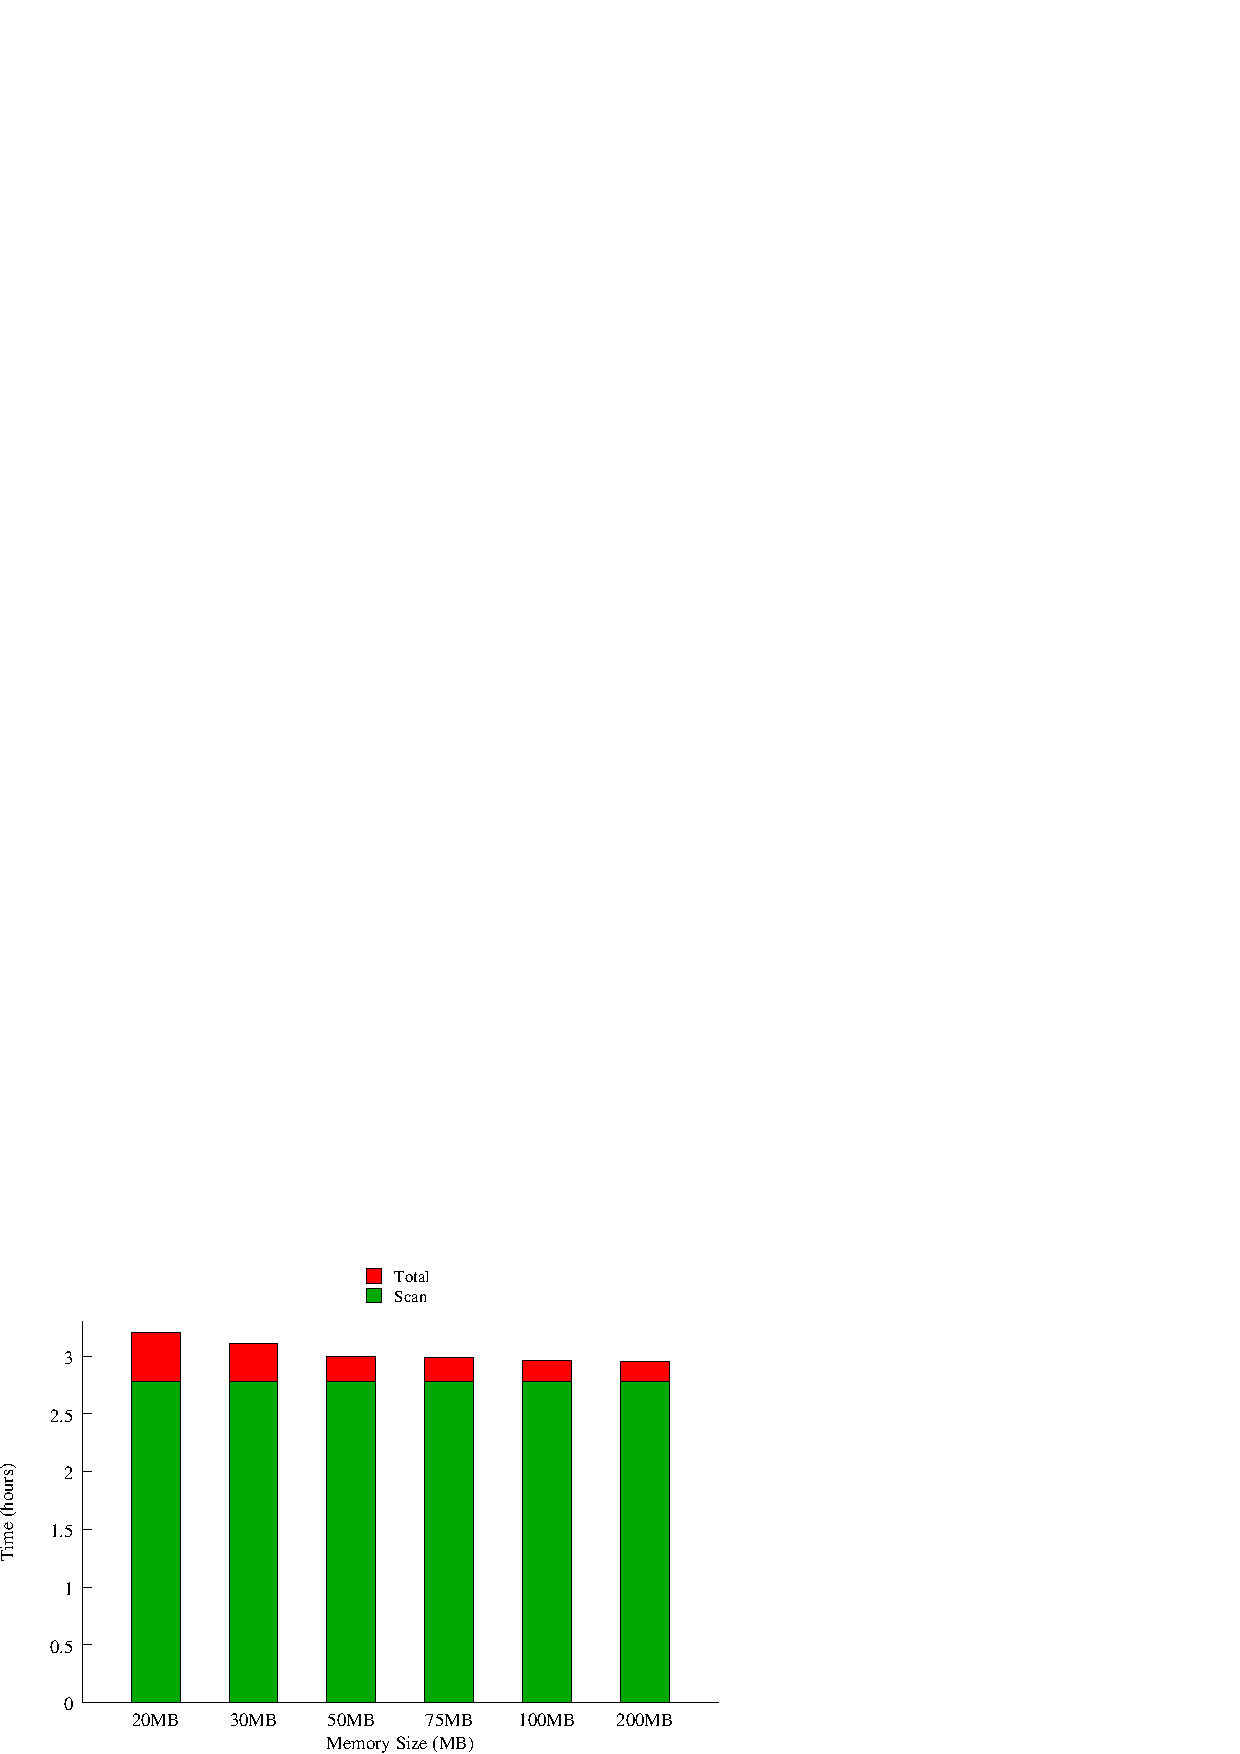
\includegraphics[width=0.4\textwidth]{mem_time.pdf}
%\caption{ Parallel time when memory limit varies.}
%\label{fig:memory}
%%\end{figure}
%
%Figure~\ref{fig:memory} shows the total parallel time in hours to backup 2500 VMs on
% a 100-node cluster a  when 


\subsection{Settings}
We have performed a trace-driven study using  a 1323 VM dataset  collected from 
100 Alibaba Aliyun's cloud nodes~\cite{WeiZhangIEEE}.
The production environment tested has  about 1000 machines with 25 VMs on each machine.
%We are running our deduplication/backup  service on 100 nodes.
%Memory usage is about 150MB space per node during backup and
%the CPU usage is very small during the experiments. 
% and each of machine nodes has 16 cores and 12 disk drives,  hosting  up to 25 VMs. 
For each VM, the system keeps 10 automatically-backed snapshots in the storage while
a user may instruct extra snapshots to be saved.
%Each VM uses   one of the most popular 7 OSes: 
%Debian, Ubuntu, Redhat, CentOS, Win2003 32bit, win2003 64 bit and win2008 64 bit. 
The backup of VM snapshots is completed within a few  hours every night.
Based on our study of its production  data,  each VM has about  40GB of storage  data usage on average
including OS and user data disk.
All data are divided into 2 MB fix-sized segments and each segment is divided into 
variable-sized content chunks ~\cite{similar94,rabin81} with an average size of 4KB.
The signature for variable-sized blocks is computed using their SHA-1 hash. 
Popularity of data blocks are collected through global counting 
and the top 1\% will fall into CDS, as discussed in Section~\ref{sect:crossVM}.
%variable sizes~\cite{similar94,rabin81} with an average size of 4KB. 
%The signature for variable-sized blocks is computed using their SHA-1 hash. 

%The seek cost of each random IO request in our test machines is about  10 milliseconds.
%The average I/O usage of local storage is controlled about 50MB/second for backup 
%in the presence of other I/O jobs. Noted that a typical 1U server can host
%6 to 8  hard drives and deliver over 300MB/second. Our setting uses 16.7\% or less 
%of local storage bandwidth. 
%The final snapshots are stored in a distributed file system built on the same 
%cluster. 

%Level 1 segment dirty bits identify 78\% of duplicate blocks. For the remaining dirty segments,
%block-wise full deduplication removes about additional 74.5\% of duplicates.
%The final content copied to the backup storage is reduced by 94.4\% in total.
%Based on the data studied,  each VM has about  40GB of storage  data usage on average,
%OS disk and data disk each takes about 50\% of storage space.
%The backup of VM snapshots is completed within two hours every day,
%and that translates to a backup throughput of 139GB per second, or 500TB per hour.
%For each VM, the system keeps 10 automatically-backed snapshots in the storage while
%a user may instruct extra snapshots to be saved.

% the system must finish saving daily snapshots of all VMs in 2 hours. In our typical 1000 nodes cluster, each node hosts 25 VMs, each VM has 40GB of data on average, that translates to backup throughput of 139GB/second, or 500TB/hour.

%In our snapshot deduplication architecture, CDS is the key to achieve greater deduplication than
%incremental backup solutions. Our basic assumption of CDS us that VM disks, especially OS disks,
%have huge amount of data in common, and such common data can be represented by a relatively smaller data set
%because of their high appearence frequency. As a result, the major portion of snapshot deduplication effect shall 
%emerge from eliminating the duplication of such a small data set. In this section, we evaluate
%the effectiveness of CDS using real user VM disks from our production VM cluster.

Since it's impossible to perform large scale analysis without affecting the VM performance,
we sampled two data sets from real user VMs to measure the effectiveness of our deduplication scheme.
Dataset1 is used study the detail impact of 3-level deduplication process,
it compose of 35 VMs from 7 popular OSes: 
Debian, Ubuntu, Redhat, CentOS, Win2003 32bit, win2003 64 bit and win2008 64 bit. For each OS, 
5 VMs are chosen, and every VM come with 10 full snapshots of it OS and data disk. 
The overall data size for this 700 full snapshots is 17.6 TB.

Dataset2 contains the first snapshots of 1323 VMs' data disks from a small cluster with 100 nodes. 
Since inner-VM deduplication is not involved in the first snapshot, this data set helps us to 
study the CDS deduplication against user-related data. The overall size of dataset2 is 23.5 TB.


\subsection{Deduplication Efficiency}

%\begin{figure}
%  \centering
%  \epsfig{file=images/overall_effect.eps, width=3.5in}
%  \caption{Impacts of 3-level deduplication. The height of each bar is the data size after 
%deduplication divided by the original data size and the unit is percentage. }
%  \label{fig:overall}
%\end{figure}

Figure~\ref{fig:overall} shows the overall impact of 3-level deduplication on dataset1.
The X axis shows the overall impact in (a),  impact on OS disks in (b), and impact on data disks in (c).
Each bar in the Y axis shows the data size after deduplication divided by the original data size.
Level-1 elimination can reduce the data size to about 23\% of original data, namely it delivers close 77\% reduction.
Level-2 elimination is applied to data that could pass level-1, it
reduces the size further to about 18.5\% of original size, namely it delivers additional 4.5\% reduction.
Level-3 elimination together with level 1 and 2
reduces the size further to 8\% of original size, namely it delivers additional 10.5\% reduction.
Level 2 elimination is more visible in OS disk than data disk, because data change frequency is really small
when we sample last 10 snapshots of each user in 10 days. Nevertheless, the overall impact of level 2 is still significant.
A 4.5\% of reduction from the original data represents about 450TB space saving for a 1000-node cluster.


%\begin{figure}
%  \centering
 %\epsfig{file=images/os_cds_sim.eps, width=3in}
%  \epsfig{file=images/3level_os.eps, width=3.5in}
%  \caption{Impact of 3-level deduplication for OS releases.}
%  \label{fig:oscds}
%\end{figure}

%To see the impact of multi-level deduplication on different OS releases,
%Some of  OS disks are modified frequently and in some cases,  users even store a large amount of user data on
Figure~\ref{fig:oscds} shows the impact of different levels of deduplication for different OS releases.
In this experiment, we tag each block in 350 OS disk snapshots from dataset1 as  ``new''
if this block cannot be deduplicated by our scheme and thus has to be written to the snapshot store;
``CDS''  if this block can be found  in CDS;
``Parent segment'' if  this block is marked unchanged in parent's segment recipe.
``Parent block'' if  this block is marked unchanged in parent's block recipe.
With this tagging, we compute the percentage of deduplication accomplished by each level.
As we can see from Figure~\ref{fig:oscds}, level-1 deduplication accomplishes a large percentage of elimination,
this is because the time interval between two snapshots in our dataset
is quite short and the Aliyun cloud service makes a snapshot  everyday  for each VM.
On the other hand,  CDS still finds lots of duplicates that inner VM deduplication can't find,
contributing about 10\% of reduction on average.

It is noticeable that level-1 deduplication doesn't work well for CentOS, a significant percentage of data is not
eliminated until they reach level-3. It shows that even user upgrade his VM system heavily and frequently
such that data locality is totally lost, those OS-related data can still be identified at level-3. 

In general we see a stable data reduction ratio for all OS varieties, ranging from 92\% to 97\%, that means
the storage cost of 10 full snapshots combined is still smaller than the original disk size. And compare to 
today's widely used copy-on-write snapshot technique, which is similar to our level-1 deduplication, our
solution cut the snapshot storage cost by 64\%.


%Combining OS disks in all the VMs, we see the overall 7.4TB of data is reduced to 512GB. 
%The extreme binning approach can reduce this data set to 542GB, which is slightly worse. As a reference, 
%perfect deduplication achieves 364GB in this experiment.

%Overall speaking, inner   VM deduplication or  CDS-based deduplication
%can work well alone, but by combining them together we get a fairly good and stable deduplication ratio to 
%all kind of OSes. 
%Compared to a traditional dirty bit approach based on pages of
%each file (e.g. segment in our scheme),
%our CDS-based level 3 approach  can save additional 50\% storage space because many of level 2 block
%content can be eliminated using the CDS also.


\subsection{Comparison with Other Approaches}
\subsubsection{Sampled Index}
One alternative approach to avoiding a single global index is to use a sampled
index. This is the approach taken by Guo and Efstathopoulos\cite{Guo2011}. We
compare their solution to ours by running their algorithm on our 350 traces
using a sampling rate of 1 out of 101 blocks, and always including the first
block in a container (which we fix at 16MB in size). The results of running this
test are shown in Table~\ref{??}, and the memory usage comparison can be found
Sec.~\ref{??}. Our results show that using a sampled index achieves a very high
rate of deduplication, and so a sampled index might be a good way to do dedup
in a single node setup.

The problems for sampling are in distributing the
algorithm and in deduplicating extremely large bodies of data. The algorithm
stores the entire (sampled) index in memory, which is required for high
throughput to avoid the disk-bottleneck problem - since the index itself has no
locality information, lookups are essentially random, so the index must be
somehow optimized to prevent excessive disk seeking (the sampling algorithm does
this by storing the index in memory). To distribute this index, each node would
either require a complete copy of the index which would have a prohibitive cost in
memory, or something like memcached must be used, which leaves the same problem
as the disk bottleneck with every index check potentially using the network.
The difficulty in storing extremely large bodies of data
is related, as once 1PB is stored in the system, assuming a sampling rate of 
1/101 with 22 byte index entires, 55GB of (in memory) index are required.

Our solution uses more total memory (??how much??), but is more scalable both in
terms of capactity and distributing the deduplication. The only part of our
algorithm which requires significant network traffic is the CDS deduplication,
but this is done after Levels 1 and 2 (dirty bits and comparison to parent), and
so is only done for a small percent of blocks (?? 5-10\% ??).

\subsubsection{Scalable Data Routing}
Another approach to avoiding a global index is to use a content-based hash
partitioning algorithm to break up the deduplication work. This approach is
taken by Dong et al. in their Scalable Data Routing paper, and is similar to
Exreme Binning\cite{??}\cite{extreme_binning09}. We compared our solution to
content-based hash partitioning by running the algorithm on our set of 
traces. We used 2MB superchunks and 4KB chunks to partition the data, and use
the minhashes of the superchunks for routing. The results of this are shown in
Table~\ref{??}. Routing each chunk to a bin provides good deduplication
efficiency, and only requires each storage node to keep an index of local data
and the bin mapping, but misses significant opportunities in our indended use
case.

The problem with the Data Routing algorithm is in the very high network traffic.
Our intended use case is a backup system which runs alongside a number of VMs,
in order to save costs. Data Routing makes no use of the inherent locality in
such a system, and therefore puts a much higher network burden on machines which
are also running 35 VMs each. This will reduce the available network bandwidth
to users of the VMs, and/or reduce the possible deduplication throughput.

